% THIS FILE IS A SELF-CONTAINED VERSION OF THE PAPER (EXCEPT FOR FIGURES)
%\documentclass[11pt,dvipdfm]{article} %dvipdfm causes a problem with blank .png figures
\documentclass[11pt]{article}

\usepackage{deauthor,times,graphicx,amsmath}
\usepackage{authblk}
\usepackage{xspace,amsmath,amsfonts}
\usepackage{wrapfig}
\graphicspath{{submissions/decision-db-abouzied/}}

%%%%%%%%%%%%% MACROS %%%%%%%%%%%%%%%%%%%%%%
\newcommand{\sql}[1]{{\small\texttt{\textup{#1}}}}
\newcommand{\attr}[1]{{\sf #1}}
\newcommand{\rel}[1]{{\sf #1}}
\newcommand{\expe}[1]{\mathbb{E}\left(#1\right)}

% Text styles (these are used for the PaQL keywords, etc.)
\newcommand{\sqlfont}{\small\selectfont\sf}
\newcommand{\sqlfontsm}{\fontsize{5.5}{4.5}\selectfont\sf}
\newcommand{\ssf}[1]{{${\sf #1}$}}
\newcommand{\bsf}[1]{{$\textsf{\textbf{#1}}$}}
\newenvironment{sqlquery}{
\sqlfont
\begin{tabbing}
\=\hspace*{0.3cm}\=\hspace*{3cm}\= \kill}%3cm
{\end{tabbing}}
\newenvironment{sqlquerysm}{
\sqlfontsm
\begin{tabbing}
\=\hspace*{1.4cm}\=\hspace*{3cm}\= \kill}
{\end{tabbing}}

% PaQL keywords
\newcommand{\SELECT}{\ssf{SELECT}\xspace}
\newcommand{\PACKAGE}[1]{\ssf{PACKAGE}(#1)\xspace}
\newcommand{\FROM}{\ssf{FROM}\xspace}
\newcommand{\REPEAT}{\ssf{REPEAT}\xspace}
\newcommand{\WHERE}{\ssf{WHERE}\xspace}
\newcommand{\SUCHTHAT}{\ssf{SUCH}~\ssf{THAT}\xspace}
\newcommand{\MAXIMIZE}{\ssf{MAXIMIZE}\xspace}
\newcommand{\MINIMIZE}{\ssf{MINIMIZE}\xspace}
\newcommand{\AS}{\ssf{AS}\xspace}
\newcommand{\AND}{\ssf{AND}\xspace}
\newcommand{\BETWEEN}{\ssf{BETWEEN}\xspace}
\newcommand{\WITHPROBABILITY}[1]{\ssf{WITH}~\ssf{PROBABILITY}~#1}
\newcommand{\EXPECTED}[1]{\ssf{EXPECTED}~#1}
\newcommand{\EXPECTEDSHORTFALL}[1]{\ssf{EXPECTED~SHORTFALL}~#1}
\newcommand{\AVG}{\ssf{AVG}}
\newcommand{\OBJ}{\ssf{OBJ}}
\newcommand{\SUM}[1]{\text{\ssf{SUM}}(#1)}
\newcommand{\COUNT}[1]{\text{\ssf{COUNT}}(#1)}

% Acronyms
\newcommand{\pb}{\textsc{PackageBuilder}\xspace}
\newcommand{\paql}{\textsc{PaQL}\xspace}
\newcommand{\spaql}{\textsc{sPaQL}\xspace}
\newcommand{\skref}{{\sc SketchRefine}\xspace}
\newcommand{\subsearch}{{\sc SummarySearch}\xspace}
\newcommand{\unitopk}{{\sf \sc TopKSketch}\xspace}
\newcommand{\SQL}{SQL\xspace}

\newenvironment{compactdesc}%
  {\begin{description}%
        \setlength{\itemsep}{0pt}
        \setlength{\parskip}{0pt}
        \setlength{\topsep}{0pt}
        \setlength{\itemindent}{0pt}
        \setlength{\leftmargin}{0pt}}%
  {\end{description}}
%%%%%%%%%%%%%%%%%%%% END MACROS %%%%%%%%%%%%%%%%%%%%%%%%

\begin{document}
    \title{In-Database Decision Support: Opportunities and Challenges}
    \author{Azza Abouzied,$^{\star}$~~~Peter J.~Haas,$^{\diamond}$~~~and~~Alexandra Meliou$\,^{\diamond}$\\
    $^{\star}$~New York University (NYU) Abu Dhabi, United Arab Emirates\\
    $^{\diamond}$~University of Massachusetts Amherst, USA}

    \maketitle
    
\begin{abstract}
    Decision makers in a broad range of domains, such as finance, transportation, manufacturing, and healthcare, often need to derive \emph{optimal} decisions given a set of \emph{constraints} and \emph{objectives}. Traditional solutions to such constrained optimization problems are typically application-specific, complex, and do not generalize. Further, the usual workflow requires slow, cumbersome, and error-prone data movement between a database and predictive-modeling and optimization packages. All of these problems are exacerbated by the unprecedented size of modern data-intensive optimization problems. The emerging research area of in-database prescriptive analytics aims to provide seamless domain-independent, declarative, and scalable approaches powered by the system where the data typically resides: the database. Integrating optimization with database technology opens up  prescriptive analytics to a much broader community, amplifying its benefits. In the context of our prior and ongoing work in this area, we discuss some strategies for addressing key challenges related to usability, scalability, data uncertainty, dynamic environments with changing data and models, and the need to support decision-making agents. We indicate how deep integration between the DBMS, predictive models, and optimization software creates opportunities for rich prescriptive-query functionality with good scalability and performance.
\end{abstract} 

%%%%%%%%%%%%%%%%%%%%%%%%%%%%%%%%%%%%%%%%%%%%%%%%%%%%%%%%%%%%%%%%%%%%%%%%%%%%
%%%%%%%%%%%%%%%%%%%%%%%%%%%%%%%%%%%%%%%%%%%%%%%%%%%%%%%%%%%%%%%%%%%%%%%%%%%%

\section{Introduction}
\label{sec:introduction}
    
\emph{Prescriptive analytics}~\cite{HaasMST11,LustigDJD10}, and constrained optimization in particular, is central to decision making over a broad range of domains, including finance, transportation, manufacturing, and healthcare. In these settings, decision makers frequently face constrained optimization problems: they need to derive \emph{optimal} decisions given a complex set of interacting \emph{constraints} and \emph{objectives}. Constraints arise from
competition between activities for scarce resources such as time, budget, workers, trucks, tools, etc., and objective functions formalize organizational goals such as minimizing costs or delays, maximizing revenue, or minimizing disease mortality.

Optimization models rely on \emph{predictive analytics}---using historical data to predict future trends as well as the future effects of current actions---in order to assess which actions will yield the best results. Predictive models can take the form of complex mechanistic simulation models that incorporate deep domain knowledge or data-driven models such as classical regression models or time series models or, more recently, machine learning models.
Moreover, \emph{descriptive analytics}---analyzing historical data to discover patterns and relationships---also plays a key role by informing the process of building optimization models so that they capture the most important relationships. Despite the fundamental interplay between
descriptive, predictive, and prescriptive analytics, the latter has received much less attention from the database community.

Modeling and solving optimization problems has typically relied on
application-specific solutions. Such solutions are often complex and do not
generalize; a decision maker seeking to apply optimization techniques in a new
application setting must either develop a new custom model from scratch, or
must learn the intricacies of generic optimization software, which can be
daunting for those with domain, but not optimization, expertise. Moreover, the
usual workflow requires that data be extracted from a database and then
reformatted and fed into a separate optimization package, after which the
output must be reformatted and inserted back into the database; this process is
slow, cumbersome, and error-prone. These challenges are further exacerbated by
the unprecedented size of modern data-intensive optimization problems.

\looseness-1
In-database prescriptive analytics is an emerging research area that aims to
provide domain-independent, declarative, and scalable approaches, supported and
powered by the system where the data relevant to these problems typically
resides: the database. This makes modeling less ad-hoc, and the overall
optimization process, from data preparation through solution and exploration of
results, becomes much more efficient. Desirable data management functionality,
such as efficient retrieval, consistency, persistence, fault tolerance, access
control, and data-integration capability, become an integral part of the system
``for free''. Interest in native DB support for prescriptive analytics has
therefore started to grow~\cite{FrazzettoDPS19}. One line of research is
exemplified by the SolveDB and SolveDB+ systems~\cite{SiksnysP16,SiksnysPNF21}.
These systems provide semi-declarative languages for specifying a broad range
of optimization problems, allow easy sharing of optimization models across
sub-problems of an overall predictive-analytics problem, and facilitate
plugging in of various prediction models and optimization-problem solvers.
\begin{wrapfigure}[11]{R}{0pt}
\centering
{\small
\begin{tabular}{clcrcc}
\attr{ID} & \attr{stock} & \attr{type} & \attr{price} & $\cdots$ & \attr{gain}\\
\hline
1  & AAPL  &Tech & 150 & $\cdots$ & ? \\
2  & MSFT  &Tech & 272 & $\cdots$ & ? \\
3  & TSLA  &Tech & 758 & $\cdots$ & ? \\
4  & AMZN  &Tech & 2400 & $\cdots$ & ? \\
5  & INTC  &Tech & 42 & $\cdots$ & ? \\
6  & GOOG  &Tech & 2280 & $\cdots$ & ? \\
7  & ADBE  &Tech & 415 & $\cdots$ & ? \\
8  & FB    &Tech & 194 & $\cdots$ & ? \\
\hline
\end{tabular}}
\vspace{-4mm}
\caption{\ssf{Stock\_Investments} table.}\label{fig:stock_investments}
\end{wrapfigure}

We have found, however, that existing solvers are often unable to deal
gracefully, if at all, with very large amounts of data, with uncertainty in the
data, with dynamic environments where the data or models are constantly
changing, or with problems that involve finding optimal policies for automated decision-making agents. Thus, the naive use of black-box solvers is often not viable for modern
large-scale optimization problems in complex environments. Our initial work aims to support the evaluation of an important class of constrained
optimization problems---integer linear programs (ILP)---within a
database~\cite{BrucatoAM18,BrucatoBAM16}. We have built a prototype system,
PackageBuilder, to specify and evaluate ILPs as ``package queries''. As a
simple example, each row of a database table might represent a food item, with
attributes describing purchase price and nutritional content. A ``package
query'' would return a ``package'' of rows (i.e., set of food items) having the
minimum possible cost while satisfying constraints on minimum required
nutritional content. More specifically, each food item~$i$ can appear $x_i$
times in the package, where each ``decision variable'' $x_i$ is a nonnegative
integer, hence the ``I'' in ILP. Both the package cost, which is to be
minimized, and the total amount of a nutrient such as vitamin D, which is
constrained to lie above a threshold, are linear functions of the $x_i$
decision variables, hence the ``L'' in ILP. Our emphasis has been on developing
fully declarative SQL extensions to specify package queries over both
deterministic and uncertain data, and to ``open up'' black box solvers in order
to develop novel scalable approximate optimization algorithms for massive,
possibly uncertain data in dynamic environments. Our work is complementary to
that in~\cite{SiksnysP16,SiksnysPNF21}, in that our techniques can potentially
be incorporated into a system such as SolveDB+.

The challenges that we consider are concretely illustrated by the following example.


\begin{example}[Investment portfolio]\label{ex:invest}
    \looseness-1
A broker wants to construct an investment portfolio for one of her clients. The client has a budget of \$50K and a planning horizon of six months. The available data comprises a table where each row corresponds to a stock. The attributes for a stock include its current purchase price per share, as well as other features such as industry sector, financial rating of the company, recent volatility, and so on; see Figure~\ref{fig:stock_investments}. 
\end{example}

% \begin{wrapfigure}[10]{R}{0pt}
% \centering
% {\small
% \begin{tabular}{clcrcc}
% \attr{ID} & \attr{stock} & \attr{type} & \attr{price} & $\cdots$ & \attr{gain}\\
% \hline
% 1  & AAPL  &Tech & 150 & $\cdots$ & ? \\
% 2  & MSFT  &Tech & 272 & $\cdots$ & ? \\
% 3  & TSLA  &Tech & 758 & $\cdots$ & ? \\
% 4  & AMZN  &Tech & 2400 & $\cdots$ & ? \\
% 5  & INTC  &Tech & 42 & $\cdots$ & ? \\
% 6  & GOOG  &Tech & 2280 & $\cdots$ & ? \\
% 7  & ADBE  &Tech & 415 & $\cdots$ & ? \\
% 8  & FB    &Tech & 194 & $\cdots$ & ? \\
% \hline
% \end{tabular}}
% \vspace{-4mm}
% \caption{\ssf{Stock\_Investments} table.}\label{fig:stock_investments}
% \end{wrapfigure}
\noindent
The ``?'' symbols indicate that the attribute \attr{gain}, which represents the gain from selling a given stock six months from now, is uncertain. The broker has available a computer model that uses the stocks' characteristics, along with other market data, to predict the joint probability distribution of stock prices six months from now. The broker wants to select a package of tuples, i.e., a portfolio of stocks, that will maximize the client's expected profit in six months, subject to the constraints that (1)~the total purchase price of the portfolio does not exceed \$50K, and (2)~the probability of losing \$1000 or more at the end of six months is at most 5\%. 

\looseness-1
As stock prices change, new stocks are added, and prediction models get updated, the optimal portfolio package may also change.  Further, as the broker discusses options with her client, they may wish to explore slight variations, e.g., \textit{what if she slightly increases or decreases her budget?} \textit{what if she increases or decreases the risk tolerance on her investment?} or, \textit{what if she wishes to eliminate or include a specific set of stocks in her portfolio?}

\smallskip
This example highlights several challenges. 
\begin{compactdesc}
    
\item[Query specification.] In our example, while the current price of a stock
may be known (deterministic), its future price is a random variable whose value
can only be described via a probability distribution. The future value of a
portfolio package is therefore also uncertain. Even in the deterministic case,
standard SQL is incapable of expressing package
constraints~\cite{BrucatoAM18,BrucatoBAM16}. In the stochastic setting,
statistical concepts such as expected values, probabilistic constraints, and
risk measures such as ``conditional value at risk'' (CVaR) compound the
specification challenge. How does one model the uncertainty of stock prices and
specify probabilistic constraints (such as bounding the risk of loss) or reason
about stochastic objectives and variables? Especially challenging is the
problem of specifying data uncertainty: probability distributions over
uncertain data values take on many different forms, including discrete,
continuous, and mixed distributions. Moreover, closed-form descriptions of
probability distributions are not always available, e.g., for financial models
of complex instruments such as ``exotic'' stock options. 

\item[Scalable processing.] Because the number of decision variables in a package query equals the number of rows in a database table, which can run to the millions, the resulting ILP is often much too large for an off-the-shelf solver to handle, even in a deterministic setting. With uncertain data, Monte Carlo methods must often be used to create an approximating ILP whose size is larger than the ILP for the deterministic case by orders of magnitude, exacerbating the problem. Indeed, a variant of the above example allows stocks to be held for varying amounts of time before sale, so that each distinct stock may be represented by multiple rows in the table corresponding to different potential sell dates; this can inflate the size of the optimization problem by more orders of magnitude.

\item[Dynamic environments.] Changes to the underlying data may be frequent, incurring expensive recomputations of the query result to keep it up-to-date. Similarly, reevaluating the packages from scratch, even for small variations of the parameters, to explore different scenarios and options, can make a what-if analysis prohibitively time-consuming.

% AZZA: Thoughts?
\item[Policy-making] As we move from one-off decisions to automated decision making by agents in time-changing and dynamic environments, the goal of prescriptive analytics shifts to construction of robust \emph{policies} that inform decisions based on (partial) observations of the current world and predictions of the future world. Consider an auto-trader that makes daily decisions about stocks to buy or sell in order to optimize for long-term gain. The auto-trader  employs an \emph{optimal} policy \emph{learned} from stock-price time-series predictions. As 
decision-making becomes increasingly autonomous, with sequential decisions in dynamic and uncertain environments, predictive and prescriptive analytics become tightly enmeshed, with \textit{reinforcement learning} methods coming into play and requiring better data management support for the massive simulated or real data sets used to constantly train predictive models, learn optimal policies and model possible outcomes.
\end{compactdesc}

In the following sections, we consider the various challenges mentioned above for in-database specification and solution of package queries. The discussion focuses on our prior and ongoing results as well as indicating directions for future work.

%%%%%%%%%%%%%%%%%%%%%%%%%%%%%%%%%%%%%%%%%%%%%%%%%%%%%%%%%%%%%%%%%%%%%%%%%%%%
%%%%%%%%%%%%%%%%%%%%%%%%%%%%%%%%%%%%%%%%%%%%%%%%%%%%%%%%%%%%%%%%%%%%%%%%%%%%

\section{Query Specification} 
    \label{sec:specification}
      
     % Query specification (PaQL and sPaQL), maybe talk about why CVAR should be considered
     
     To allow declarative specification of package queries in a DBMS-friendly manner, a natural approach is to extend the \SQL language to support such queries. We first introduce \paql, our \SQL extension for declarative specification of deterministic package queries, and then discuss further extensions to handle data uncertainty, leading to the \spaql language extension.
     
\subsection{Package Query Language (PaQL)}\label{sec:paql}

The \paql language extension allows users to declaratively express combinatorial optimization problems with linear objectives and constraints natively within a relational database.
% The following is an example of a package query:

\begin{example}[Meal Plan]
    \label{ex:meal-plan}
    A dietitian needs to design a meal plan for a patient.
    She wants three distinct gluten-free meals, between 2K and
    2.5K calories in total, and with a low total intake of
    saturated fats. Each row in the relational table \sql{Recipes} describes a distinct meal, giving the total number of calories and total amount of saturated fats and gluten, along with other nutritional information.
\end{example}

Package queries extend traditional database queries by allowing users to not only express
standard selection constraints (e.g., each meal must be gluten-free),
but also higher-order \emph{package-level} constraints
(e.g., all meal plans must have between 2,000 and 2,500 calories in total)
and objectives (e.g., minimize the meal plan's total saturated fat).
The Package Query Language (\paql) extends \SQL to allow for their declarative expression.
The Meal Plan query in Example~\ref{ex:meal-plan} can be expressed in \paql as follows:

\begin{sqlquery}
\hspace*{5mm}\=\hspace*{1.8cm}\=\hspace*{1.3cm}\= \kill%1.8cm
\>\SELECT         \>\PACKAGE{$\ast$} \\
\>\FROM           \>\rel{Recipes} \REPEAT $0$ \hskip 1em/* each meal can appear at most once in a package */\\
\>\WHERE          \>$\attr{gluten} = 0$ \\[2pt]
\>\SUCHTHAT       \\
\>\>$\COUNT{\ast} = 3$ \AND \\[2pt]
\>                \>\SUM{\attr{kcal}} \BETWEEN $2.0$ \AND $2.5$\\[2pt]
\>\MINIMIZE       \>$\SUM{\attr{sat\_fat}}$
\end{sqlquery}

The PackageBuilder system transforms a \paql specification into an ILP and uses
an off-the-shelf ILP solver to compute the desired package. When, as is
typical, the number of database rows is large, direct solution by the solver is
infeasible because of the large size of the ILP. We have developed an iterative
approximate solution algorithm called \skref~\cite{BrucatoBAM16} (discussed in
Section~\ref{sec:scalability}) to handle large numbers of rows while providing
approximation guarantees.

\subsection{sPaQL}\label{sec:spaql}

In preliminary work~\cite{BrucatoMAHM20,BrucatoAHM2020}, we have started to extend PackageBuilder to handle uncertain data. 
Dealing with uncertainty is crucial, because uncertain data is pervasive. For
example, data values might represent outputs of predictive stochastic models as
in the stock examples, or might derive from noisy processes such as sensor
readings, privacy shielding, data integration, or extraction of structured data
from text, images, or video~\cite{suciu2011probabilistic}. Thus, decisions must
often be made in the face of uncertainty, i.e., the decision maker must solve a
\emph{stochastic optimization problem}.
As a first step, we have extended  \paql to allow specification of \emph{stochastic package queries (SPQs)}; the extended language is called \spaql. For example, the portfolio-selection problem of Example~\ref{ex:invest} can be expressed in \spaql as follows:
% 
\begin{sqlquery}
\hspace*{5mm}\=\hspace*{1.8cm}\=\hspace*{1.3cm}\= \kill
\>\SELECT         \>\PACKAGE{$\ast$} \AS Portfolio\\
\>\FROM           \>\rel{Stock\_Investments} \\
\> \WHERE       \> \attr{type} $=$ \ssf{'Tech'}\\
\>\SUCHTHAT \\
\>\>$\SUM{\attr{price}} \le 50{,}000$ \AND\\
\>\>$\SUM{\attr{gain}} \ge -1000$ \bsf{WITH PROBABILITY} $\ge 0.95$\\[4pt]
\>\MAXIMIZE       \>\bsf{EXPECTED} $\SUM{\attr{gain}}$
\end{sqlquery}

\noindent A \spaql query such as the one above specifies a \emph{stochastic} ILP (SILP) whose solution is the desired package. Expected-value constraints such as \EXPECTED $\SUM{\attr{attr}} \ge x$ are also allowed.

%%%%%%%%%%%%%%%%%%%%%%%%%%%%%%%%%%%%%%%%%%%%%%%%%%%%%%%%%%%%%%%%%%%%%%%%%%%%
%%%%%%%%%%%%%%%%%%%%%%%%%%%%%%%%%%%%%%%%%%%%%%%%%%%%%%%%%%%%%%%%%%%%%%%%%%%%

\section{Scalable Query Evaluation}
    \label{sec:scalability}
    
    %MCDB approach of stochastic predictive models as VG functions, can also do this with deterministic predictive models
    
   % Summarize our old results, say that we are working on joint scalability for SPQs.
   
In this section, we provide an overview of scalable evaluation methods for
package queries (PQs). Scalability challenges arise in the presence of large
datasets and are further exacerbated by the use of Monte Carlo methods for
solving stochastic package queries (SPQs); the latter methods require
generation of multiple ``scenarios''. We discuss the \skref algorithm for
addressing the first challenge in the context of deterministic PQs and then
discuss an algorithm called \subsearch for scalability with respect to
scenarios. We then outline the challenges of bringing these two research
threads together to evaluate SPQs over large sets of uncertain data.
   
      \begin{figure}[t!]
    \centering
%    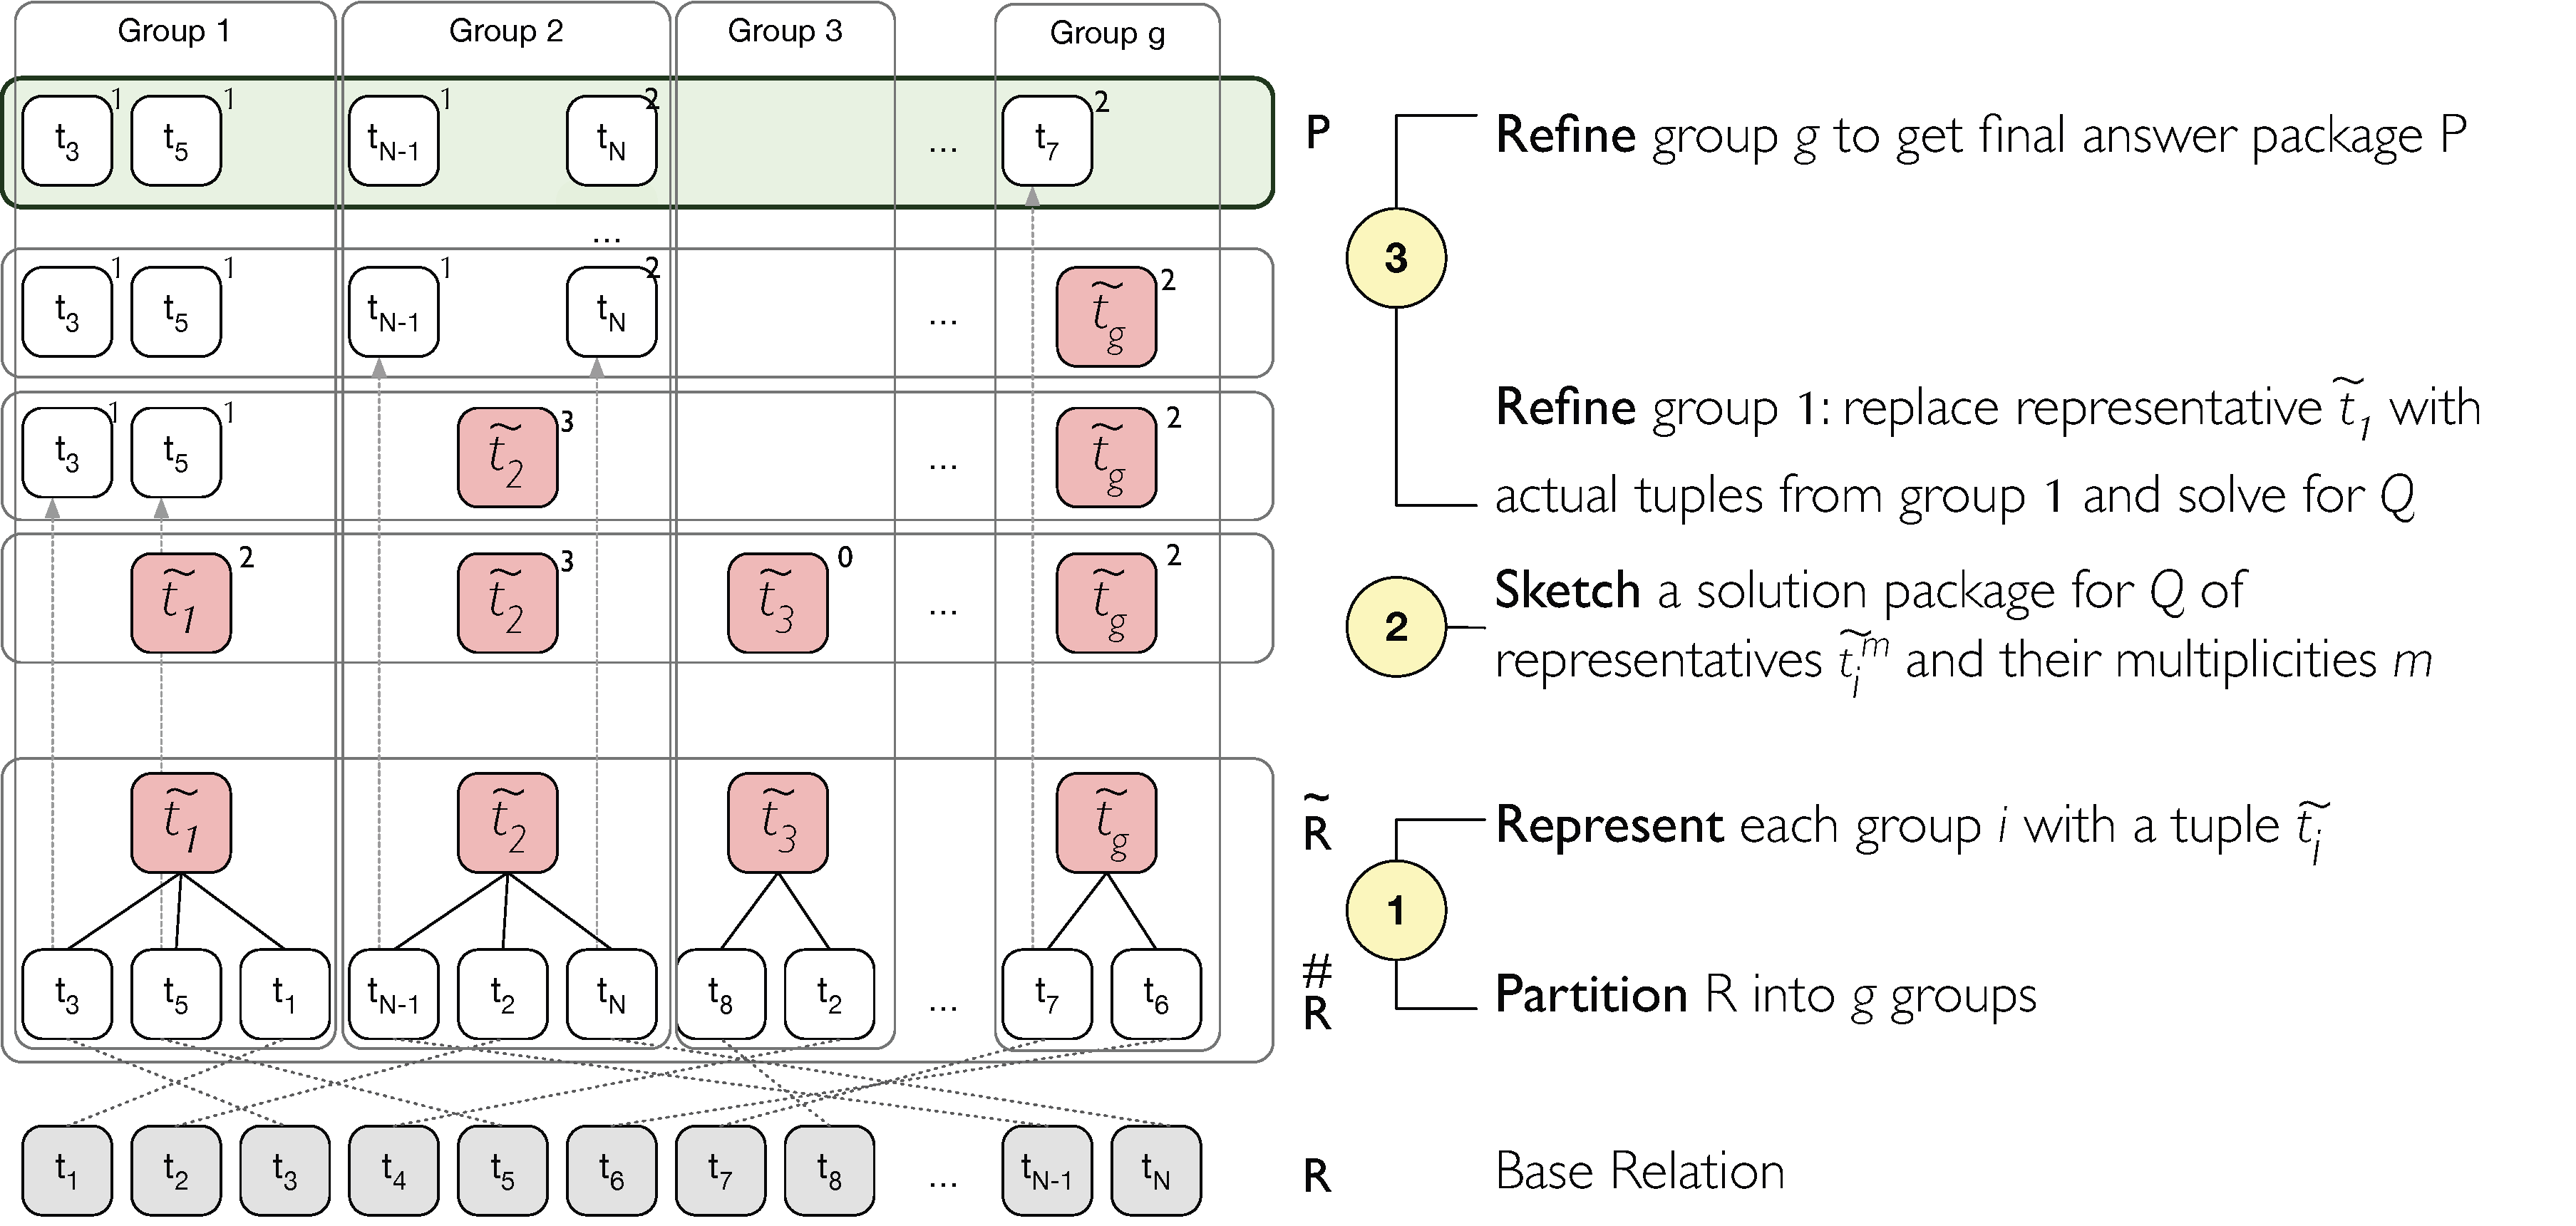
\includegraphics[width=1\textwidth]{figs/SketchRefine.png}
    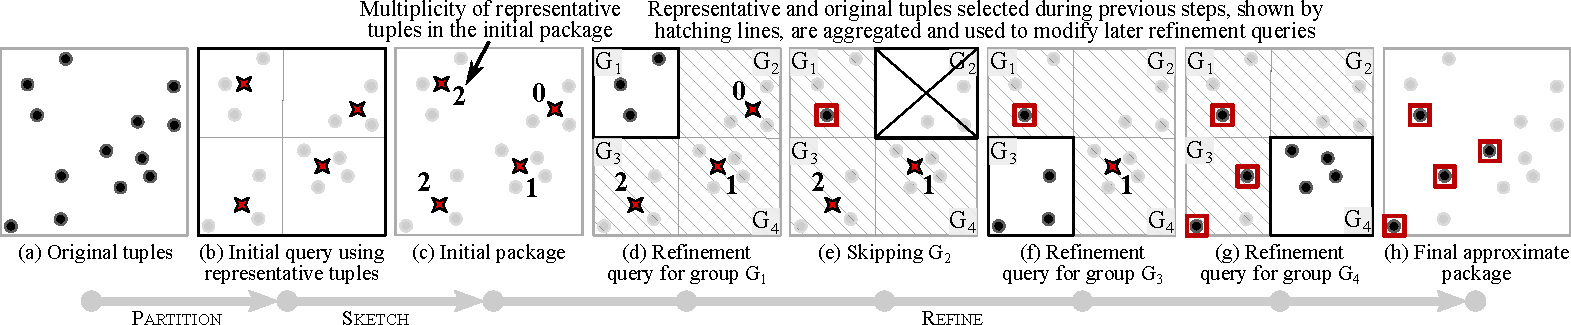
\includegraphics[width=1\textwidth]{figs/explain4.pdf}
        %\vspace{-6mm}
%    \caption{An illustration of the \skref algorithm.}
    \caption{An illustration of the \skref algorithm. The original tuples (a) are partitioned into four groups and a representative is constructed for each group (b). The initial sketch package (c) contains only representative tuples, with possible repetitions up the size of each group. The refine query for group $G_1$ (d) involves the original tuples from $G_1$ and the aggregated solutions to all other groups ($G_2$, $G_3$, and $G_4$). Group $G_2$ can be skipped (e) because no representatives could be picked from it. Any solution to previously refined groups are used while refining the solution for the remaining groups (f and g). The final approximate package (h) contains only original tuples. (Figure taken from \cite{BrucatoBAM16}.)}
%    \vspace{-2mm}
    \label{fig:sketchrefine}
\end{figure}

   \subsection{Scaling Deterministic Package Queries with SketchRefine}
   \label{sec:pql}

   The PackageBuilder system transforms a \paql specification into an ILP and uses an off-the-shelf ILP solver to compute the desired package. When, as is typical, the number of database rows is large, direct solution by the solver is infeasible because of the large size of the ILP. In prior work, we developed an iterative approximate solution algorithm called \skref~\cite{BrucatoBAM16} to handle large numbers of rows while providing approximation guarantees. Briefly, the algorithm first partitions the rows into groups, where the rows in each group have similar attribute values, and then computes a representative for each group. A small ILP using only the representatives can be then easily solved---the ``sketch''. The sketch is then iteratively ``refined'' by carefully replacing each representative using the rows that it represents.  The process maintains feasibility of the current solution until the final package is obtained. Limiting the size of each group to be a small number of $\tau$ tuples ensures that each refine phase can be executed efficiently and allows for approximation guarantees. Figure~\ref{fig:sketchrefine} illustrates the three key operations of \skref: partition, sketch and refine.
   
\subsection{Scaling Stochastic Package Queries with Respect to Scenarios}
   \label{sec:spqNew}
   
Evaluating SPQs is very challenging, due to the sheer size of the optimization problems: First, as with deterministic PQs, there is a decision variable for every row of a (potentially very large) table. Second, the presence of uncertainty typically requires multiple versions of the table, called scenarios, that represent Monte Carlo realizations of the uncertain data values. Often, a large number of scenarios is required for accuracy, inflating the problem size by orders of magnitude. 

\smallskip\textit{Exact evaluation:} One approach tackles the scalability challenge of stochastic problems by eliminating uncertainty. E.g., it is indeed possible to translate a stochastic package query into an integer program when (i)~the expected value of each attribute in an expectation objective is known and (ii)~each attribute in a probabilistic constraint has a Gaussian distribution with known mean and variance. It is possible to derive precise rules that enable this translation. Consider, for example, an expectation objective on attribute $\attr{A}_j$, i.e., the goal is to minimize the expected value of the sum of $\attr{A}_j$ over all tuples in the package. The objective function to be minimized takes the form $\expe{\sum_i A_{ij}\cdot  x_i}$. Because of the linearity of expectation, $\expe{\sum_i A_{ij}\cdot x_i} = \sum_i \expe{A_{ij}}\cdot x_i = \sum_i t_i.{\mu\attr{A}_j} \cdot x_i$, where \ssf{t_i.\mu\attr{A}_j} is the expected value of $\attr{A}_j$ for tuple $t_i$. Therefore, we can simply replace the expectation objective with a linear deterministic objective. Similarly, linear Gaussian probabilistic constraints can be transformed into deterministic quadratic constraints; we require, however, that the resulting constraints be convex.

\begin{figure}[t!]
\centering
\begin{tabular}{ccr}
\multicolumn{3}{c}{\textbf{Scenario 1}}\\[4pt]
\attr{ID} & $\cdots$ & \attr{gain}\\
\hline
1  & $\cdots$ & 20\\
2  & $\cdots$ & 3\\
3  & $\cdots$ & -30\\
4  & $\cdots$ & 10\\
5  & $\cdots$ & 200\\
6  & $\cdots$ & -10\\
7  & $\cdots$ & 30\\
8  & $\cdots$ & 20\\
\hline
\end{tabular}
\hskip 3em
\begin{tabular}{ccr}
\multicolumn{3}{c}{\textbf{Scenario 2}}\\[4pt]
\attr{ID} & $\cdots$ & \attr{gain}\\
\hline
1  & $\cdots$ & 10\\
2  & $\cdots$ & 6\\
3  & $\cdots$ & -5\\
4  & $\cdots$ & 4\\
5  & $\cdots$ & 120\\
6  & $\cdots$ & -20\\
7  & $\cdots$ & 15\\
8  & $\cdots$ & 16\\
\hline
\end{tabular}
\hskip 3em
\begin{tabular}{ccr}
\multicolumn{3}{c}{\textbf{Scenario 3}}\\[4pt]
\attr{ID} & $\cdots$ & \attr{gain}\\
\hline
1  & $\cdots$ & -2\\
2  & $\cdots$ & 8\\
3  & $\cdots$ & -25\\
4  & $\cdots$ & 36\\
5  & $\cdots$ & 70\\
6  & $\cdots$ & 15\\
7  & $\cdots$ & 20\\
8  & $\cdots$ & 7\\
\hline
\end{tabular}
\hskip 4em
\begin{tabular}{ccr}
\multicolumn{3}{c}{\textbf{Summary}}\\[4pt]
\attr{ID} & $\cdots$ & \attr{gain}\\
\hline
1  & $\cdots$ & -2\\
2  & $\cdots$ & 3\\
3  & $\cdots$ & -30\\
4  & $\cdots$ & 4\\
5  & $\cdots$ & 70\\
6  & $\cdots$ & -20\\
7  & $\cdots$ & 15\\
8  & $\cdots$ & 7\\
\hline
\end{tabular}
\caption{Three example scenarios and a summary for the \ssf{Stock\_Investments} table.}
\label{fig:threescenarios}
\vspace{-3mm}
\end{figure}

\smallskip
%\looseness-1
\emph{Monte Carlo evaluation:} The foregoing method has the great benefit of being exact, but has  limited applicability and may fail even on small problems (few rows) because of the complexity of the quadratic constraints. In preliminary work, we have developed a more general strategy based on Monte Carlo (MC) sampling. The idea is to approximate the SILP with a deterministic ILP. Specifically, we replace the expectation objective with an empirical average over a set of randomly generated \emph{scenarios}, and similarly replace a probabilistic constraint---e.g., that an inequality be satisfied with 90\% probability---with a requirement that, e.g., the inequality hold for 90\% of the scenarios. This approach forgoes exact optimality in order to (1)~allow arbitrary distributions for random variables appearing in probabilistic constraints, (2)~avoid the convexity requirements on probabilistic constraints mentioned previously, (3)~allow correlation between tuples, and (4)~obtain less complex (i.e., not quadratic) constraints. The only requirement is the ability to sample values from each random variable. To this end, we can store uncertain data in a probabilistic database~\cite{suciu2011probabilistic}, specifically a ``Monte Carlo database system'' such as MCDB or SimSQL~\cite{AJP+10,Cai+13,JampaniXWPJH11,JampaniXWPJH08,PerezAJ10},
which offer support for arbitrarily complex random distributions of the kind needed to
support optimization problems such as portfolio selection. Roughly speaking, the uncertainty of a given data item is specified via a user-defined \emph{value generation (VG) function} which, when invoked, generates a sample realization of the data-item value from its underlying probability distribution. VG functions can generate values for multiple data items simultaneously, thereby allowing complex statistical correlations between data items. By evaluating every VG function in a table, we get a sample realization of the table, which we call a \emph{scenario}. (Scenarios are also called ``possible worlds'' in the literature on probabilistic databases.) Figure~\ref{fig:threescenarios} shows three possible scenarios (the leftmost three tables) for the table in Figure~\ref{fig:stock_investments}. After computing an optimal package, its true feasibility and objective value for the original SILP can be determined to high accuracy using a very large number of ``validation'' scenarios; this calculation is much faster than solving the approximate ILP optimization problem.

The deterministic ILP obtained as described above is called a \emph{stochastic average approximation (SAA)} and approximates the SILP. Often, many scenarios are required to obtain a sufficiently accurate approximation. Indeed, if too few scenarios are used, then the solution to the SAA will be infeasible for the true SILP, but will have an objective value that is better than the true one, so that we think that we are doing better than we actually are; this phenomenon is known as the ``optimizer's curse''~\cite{smith2006optimizer}. The size of the SAA is proportional to the number of database rows times the number of scenarios, which makes direct use of an off-the-shelf solver infeasible.

\smallskip\textit{Scaling the number of scenarios:} To address this scalability problem, we developed an algorithm called \subsearch~\cite{BrucatoAHM2020} that can drastically reduce the number of scenarios required. \subsearch replaces the large set of scenarios used to form the SAA by a very small synopsis of the scenario set, called a \emph{summary}, which results in a reduced ILP, called a \emph{conservative summary approximation (CSA)}, that is much smaller than the SAA. A summary is carefully crafted to be ``conservative'' in that the constraints in the CSA are harder to satisfy than the constraints in the SAA, thereby pushing the solver to find truly feasible solutions. In our portfolio example, a summary of a set of three scenarios can be obtained by taking the row-wise minimum of the gains as shown in Figure~\ref{fig:threescenarios}; if the gain of a package with respect to the summary exceeds $-\$1000$, then clearly the gain of 100\% of the original three scenarios exceeds $-\$1000$. By taking the row-wise minimum over more or fewer random scenarios, the summary can be made more or less conservative.

\looseness-1
Because the ILP for the CSA is much smaller than that for the SAA, it can be solved much faster. Moreover, the resulting solution is much more likely to be truly feasible (as verified using a large set of validation scenarios), so that the required number of optimization/validation iterations is typically reduced. Of course, if a summary is overly conservative, the resulting solution will be feasible, but highly suboptimal. Therefore, during each optimization phase, \subsearch implements a sophisticated search procedure aimed at finding a ``minimally'' conservative summary; this search requires solution of a sequence of reduced ILPs, but each can be solved quickly. In experiments reported in \cite{BrucatoAHM2020}, \subsearch was able to answer SPQs faster by orders of magnitude than the prior approach of sequentially adding more and more scenarios to an SAA until either the solution package is truly feasible (as measured by the validation set) or the solver chokes; indeed, \subsearch was able to compute good, truly feasible solutions in many cases where the prior approach would fail. 

\subsection{Fully Scaling Stochastic Package Queries}
   \label{sec:spqSR}

The \subsearch algorithm addresses the scalability issue with respect to the number of scenarios, but does not address scalability with respect to the number of database rows. For interactive decision making in dynamic, uncertain environments involving large amounts of data, both issues must be addressed simultaneously. In current work, we are extending our SPQ evaluation algorithms to handle large numbers of database rows. A promising direction is to use a sketch-and-refine approach as an ``outer loop'' to generate a sequence of SILP problems with a small number of rows which are solved using techniques that are scalable in the number of scenarios. To further improve speed and efficiency, a potentially powerful approach opens the lid on the ILP solver to try and exploit the characteristics specific to ILPs in the package-query setting.

\smallskip
%\looseness-1
\emph{Adapting and improving SketchRefine:} As with \skref for deterministic data, we create the sketch by replacing the rows with a small set of representatives and then subsequently refine it. A key question is how to define the partitions and compute the representatives. In the deterministic setting, the distance between rows, which can be viewed as points in a multidimensional space $S$ of attribute values, is relatively straightforward to define. In the stochastic setting, each row represents a multidimensional \emph{probability distribution} over $S$. This raises the question of how to appropriately define distances between the stochastic rows. There are many distance metrics for probability distributions, and for any metric there is an trade-off between space requirements, accuracy, and computational cost when estimating the metric from scenarios. Possible approaches include estimating a metric using raw samples, histograms, quantiles, or kernel-density methods~\cite{silverman2018density}. It is also desirable to parallelize the partitioning operation, which cannot be easily done in the prior clustering-based approach used in \skref; we are therefore currently investigating alternative divide-and-conquer approaches. In addition, it is often the case that multiple data items use the same choice of VG function, perhaps with slightly varying parameterizations, to generate samples when creating a scenario; this information can potentially be exploited to develop effective partitioning schemes. Once a partition is determined, a (stochastic) representative can potentially be computed in a number of different ways, varying in accuracy and computational effort.

\begin{wrapfigure}[25]{R}{0pt}
    \centering
    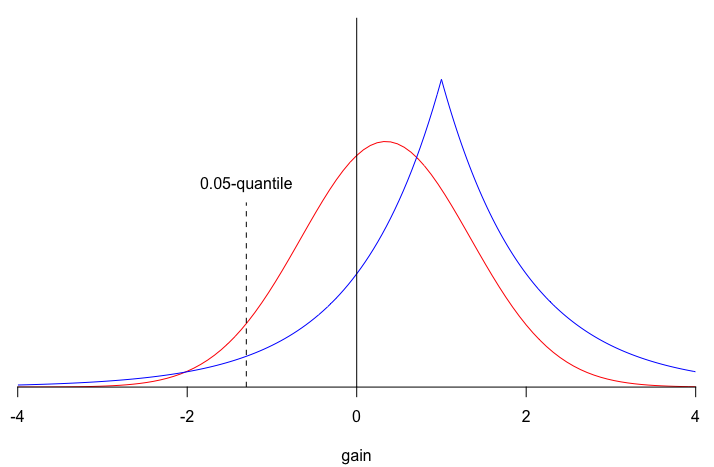
\includegraphics[scale=0.3]{figs/CVARexample.png}
    \caption{Two plots visualizing the probability distributions of the total gains of two different packages. The blue curve denotes a package with a higher expected sum, but in its lower 5\% of cases, the average loss is almost three times higher than that of the red curve. VaR constraints alone do not differentiate between the two plots, since the right boundary of the lower 5\% tail is the same in both distributions. CVaR constraints allow users to limit the expected loss in the tail of the distribution, and avoid high-risk packages such as one shown in blue.}
    \label{fig:cvar_motivation}
\end{wrapfigure}
For the inner loop, we are investigating improvements to \subsearch by exploiting the tractability of \emph{CVaR constraints}. 
The probabilistic constraint on the gain in the \spaql query in Section~\ref{sec:spaql} is called a \emph{chance constraint} in the stochastic-programming literature. In risk-management terminology~\cite{McNeilFE15}, the $\alpha=0.95$ \emph{Value at Risk} (VaR) is \$1000 in the worst case; that is, the probability of losing \$1000 or more is at most $1-\alpha=5\%$. Although VaR is a widely used risk measure, it has a number of deficiencies. Intuitively, knowing that there is at most a 5\% chance of losing \$1000 \emph{or more} is not totally reassuring, since the actual loss in the bad 5\%-probability scenario---i.e., the ``worst 5\% of cases''---is not controlled at all. Risk analysts are increasingly preferring to supplement or replace the VaR measure of risk with an alternative measure, called the \emph{Conditional Value-at-Risk} (CVaR)---also called \emph{Expected Shortfall}---with confidence $\alpha$, defined as the expected loss given that the loss exceeds the $\alpha$-VaR. Unlike VaR, the CVaR measure has the desirable ``subadditivity'' property that bounds the total risk of a set of gambles by the sum of the individual risks, thereby encouraging risk reduction through diversification, unlike VaR.

As indicated in our discussion of exact evaluation methods in Section~\ref{sec:spqNew}, a constraint defined in terms of an expected value can be converted to a simple linear constraint that is relatively easy to handle. In a similar manner, a CVaR constraint, since it comprises an expectation, can also be handled much more easily than a VaR constraint. Interestingly, it appears as if a problem with a VaR constraint can be solved by rapidly solving a sequence of problems involving only CVaR constraints, avoiding the need to search for appropriately conservative summaries. 

\smallskip

\emph{Re-engineering the ILP solver:} The ILP solver plays a key role in solving both deterministic and stochastic package queries, so speeding up the solver module can significantly  improve the performance of all methods discussed so far. Moreover, in the setting of \skref, a solver that can scale to large numbers of rows reduces the number of refinement steps required and improves accuracy. An important characteristic of the ILP problems that arise in our setting is that the number of rows $n$ is much larger than the number of constraints $m$, since constraints are typically manually defined by the user whereas the number of rows equals the table cardinality. This creates opportunities to replace a general-purpose ILP solver by a specially designed paralellizable approximate ILP solver (A-ILP), which can speed up processing not only of SPQs, but also of deterministic package queries and more general ILPs having a high $n$-to-$m$ ratio. In preliminary work, we have started to develop such an improved solver. The rough idea is to first relax the ILP to a linear program (LP) by dropping the integrality constraints. The LP is then solved using a novel variant of the well known dual-simplex algorithm~\cite{vanderbei2020linear} that exploits the $n$-to-$m$ ratio in multiple ways for speed and efficiency. An $O(m+\log n)$ ``guided lattice walk'' is then used to obtain a reduced ILP with fewer variables that approximates the original ILP. The reduced problem is then solved exactly by a standard ILP solver. Initial experiments on an 8-core machine show that the A-ILP solver can have an accuracy comparable to the commercial Gurobi ILP solver while being twice as fast; the relative speed-up is expected to become even more pronounced as the number of cores increases due to the parallelizability of the novel dual-simplex algorithm. We also found that A-ILP scales well, approximately solving an ILP with tens of millions of variables in 5--8 seconds. We intend to theoretically analyze the properties of A-ILP and leverage it to enhance interactivity in \pb.

%%%%%%%%%%%%%%%%%%%%%%%%%%%%%%%%%%%%%%%%%%%%%%%%%%%%%%%%%%%%%%%%%%%%%%%%%%%%
%%%%%%%%%%%%%%%%%%%%%%%%%%%%%%%%%%%%%%%%%%%%%%%%%%%%%%%%%%%%%%%%%%%%%%%%%%%%
    
\section{Dynamic Data and Models} 
    \label{sub:changing_data_and_models}
    
Another key challenge for in-database optimization via package queries is that,
even for small delta changes in the underlying data or in the query parameters,
the computationally intensive package query needs to be re-executed from
scratch. Yet, in most real-world applications, the overall form of the
constrained optimization problem remains roughly the same, while the data or
the query parameters incrementally change often within short time spans. The
requirement to re-execute such queries from scratch makes maintaining results
up-to-date computationally tedious and exploratory analysis impractical. In
this section, we sketch some ideas for performing \emph{incremental maintenance}
of package results when the underlying data or query parameters change slightly
in order to support interactive exploration and analysis. We discuss
deterministic data first, and then extend our discussion to stochastic data.

\subsection{Incremental PQ maintenance under data perturbations}
\label{sec:deltaData}

Incremental package maintenance under data changes can be handled heuristically: Let $P$ be the set of tuples appearing in a package result, $R$ the set of tuples that were deleted from the original database $D$, and $A$ the set of tuples that were added to $D$. A heuristic solution to the standing package query can be obtained by running it on the dataset $(P\setminus R)\cup A$.  Assuming that the data change is small, this should be a small set of tuples, over which one can solve the constrained optimization problem directly. This method can serve as a heuristic baseline; a more principled approach rests on a modification of the \skref algorithm.

The \skref algorithm provides package solutions that are a $(1\pm\epsilon)$-factor close to the optimal solution. It achieves this tight approximation bound by ensuring that each partition or group has a maximum diameter $\omega$ such that $\omega$ depends on $\epsilon$ and all tuples in the group are within a radius $\omega/2$ of the group's centroid or its representative tuple. Given this theoretical guarantee of \skref's behavior, we identify the \textit{irrelevant tuples} of an incremental update as inserted tuples  ($\Delta R$) that can be placed into an existing group without violating its diameter $\omega$ or size $\tau$ limits, or deleted tuples ($\nabla R$) that do not occur in the solution package. 

A scalable incremental \skref variant can potentially employ an incremental tree index to maintain tuple-group mappings and can easily split groups that exceed the diameter or size limits. In this way, recomputations are only triggered when an incremental update causes a tree restructuring. Moreover, since partitioning and representative tuple construction is incrementally maintained, only parts of the \skref algorithm need to be re-executed and not the entire algorithm for certain updates. For example, when a tuple appearing in the solution package is deleted from the base relation, we only need to re-refine the group to which the tuple previously belonged.

Additionally, one can potentially exploit the fact that the A-ILP solver described in Section~\ref{sec:spqSR} hinges on the dual-simplex algorithm. This algorithm is known to be amenable to incremental processing, and could potentially be leveraged for incremental package updating.

\subsection{Incremental PQ maintenance under query perturbations}
\label{sec:deltaQuery}

A decision-maker may wish to quickly determine the effect of changing some query parameters on the overall objective value. For example in the meal planning query (Example~\ref{ex:meal-plan}), \emph{`does relaxing the constraint on calories lead to a lower-fat plan and to what degree}'? Often, a rapid, initial estimate of the objective value and an approximate, feasible, package solution is sufficient to help the decision-maker decide on whether they wish to settle on the new query parameters, in which case, the new query can be fully and accurately evaluated.

We identify five practical mechanisms for interactive query refinements: (i)~changing the threshold parameters of base constraints to tighten or relax a query, (ii)~tuple exclusions or tuple inclusions, (iii)~changing the threshold parameters of global constraints, (iv)~converting base constraints to global ones and vice versa, and (v)~in the case of stochastic package queries changing the chance or CVaR parameters associated with a constraint. An interesting research challenge is to  develop one or more scalable evaluation techniques that provide an upper-bound (lower-bound) estimate of the objective value for minimization (maximization) queries and an initial feasible package interactively. Heuristic methods can avoid making expensive calls to the integrated ILP solver and rely instead on efficient database top-k querying techniques. This is necessary to ensure sub-second response times that are crucial for exploratory interactive query refinement such as when a user drags a slider to control the threshold values of selection constraints: as they drag the slider, they would like to immediately understand the impact of their refinement on the objective value and overall package solution.

We briefly describe a promising heuristic, \unitopk, that we hope to expand and analyze.  \unitopk computes and maintains an ordered list of tuples in each \skref partition: the ordering is determined by both the objective function and the selection constraints of the package query. The ordered lists are similar to an onion index~\cite{onion}. On query refinement, we select the top-k tuples from each ordered list that satisfy the refined selection constraints. Along with the original package, we pass these new tuples to the solver to recompute a solution. This approach avoids the repeated refine operations (as a solution is built on actual tuples and not representative tuples) and is equivalent in complexity to a single sketch operation. In preliminary experiments, we found this approach to return results interactively ($< 20$ ms) for the refinements discussed above with near-optimal objective values.

\subsection{Incremental SPQ maintenance}\label{sec:incSPQ}

Perturbations to data and queries occur in the stochastic setting as well. For example, in the portfolio problem, an investor might originally only have considered NYSE stocks but may now also want to consider Nasdaq stocks. Should she replace some NYSE stocks with Nasdaq stocks in her previously optimal portfolio? The degree of risk than she might tolerate may change over time as her financial position or other factors change. Perhaps she wants to understand the effect on the expected gain from her ``optimal'' portfolio if interests rates turned out to be somewhat higher than the stock-prediction model originally assumed; is a modified portfolio needed? 

\looseness-1
The techniques discussed in Section~\ref{sec:deltaQuery}, such as \unitopk, focus on incremental maintenance for deterministic package queries under small perturbations such as tightening or loosening constraints and adding or removing rows. Since these techniques essentially focus on updating the solution to an ILP, they are also potentially applicable, perhaps with modifications, for updating the solution to the types of ILP used in the various methods for SPQ evaluation. However, there are aspects of incremental maintenance that are unique to SPQs. In particular, even if the query and the set of stochastic database rows (e.g., stocks) stays the same, a user might want to experiment with the underlying probability distribution of the uncertain data values. In particular, a predictive stochastic model used to generate scenarios often involves a vector $\theta$ of parameters that a user might want to vary. For example, a predictive stock-price model might assume certain values for interest and unemployment rates, and the user might want to see how the optimal portfolio changes when these parameters are varied. If the parameters are not perturbed too much, are there good ways of leveraging prior optimization results?

\smallskip\textit{Quick updates via stochastic search:} When the parameter changes are relatively small, it may be advantageous to update the current package using a stochastic search algorithm designed for noisy observations, such as adapted versions of simulated annealing~\cite{alkhamis2004simulation,alrefaei1999simulated} and genetic algorithms~\cite{xiao2014simulation}, or other algorithms such as stochastic ruler~\cite{alrefaei2005discrete}, 
%adaptive hyperbox~\cite{xu2013adaptive},
branch-and bound~\cite{norkin1998branch}, and so on. The motivation is that such algorithms are designed to minimize the number of scenarios needed and can search though nearby packages rapidly, with no calls to a solver, while also using stochasticity to avoid getting trapped in a local optimum.

\smallskip\textit{Fast sensitivity analysis:} Another potentially effective enabler of interactivity is to compute gradient information at the same time that we compute scenarios in order to allow a user to quickly evaluate the effect of small changes in $\theta$. Given a package $\mathcal P$, a typical objective function has the form $H_\theta(\mathcal{P})=\sum_{j\in\mathcal{P}}E_\theta[g(A_j,\theta)]$ for a given random attribute $A$. For example, $A_j$ might be the random gain for the $j$th stock, $\theta$ might be the interest rate used in the predictive model, and $g(x,\theta)$ might be a function that computes the net present value (NPV) of the gain. The subscript $\theta$ on the expectation operator $E$ indicates that the the interest rate affects the predicted NPV of the gain not only explicitly through the function $g$, but also implicitly by affecting the probability distribution of the random variable $A_j$. For simplicity, suppose that the random variable $A_j$ has a known probability density function $f_\theta$. Under mild regularity conditions, it is known~\cite{glynn1990likelihood} that $\nabla_\theta E_\theta[g(A_j,\theta)]=E_\theta[Y_j]$, where $Y_j=g'(A_j,\theta)+g(A_j,\theta)L'(0)$, $g'=\partial g/\partial \theta$, and $L(h)= f_{\theta+h}(A_j)/f_\theta(A_j)$. The quantity $L$ is a \emph{likelihood ratio} for $A_j$. We then find that $\nabla_\theta H_\theta(\mathcal{P}) =\sum_{j\in\mathcal{P}}E_\theta[Y_j]$. Thus when generating a scenario value of $A_j$, we can simultaneously compute the quantity $Y_j$. Averaging the $Y_j$ values over all of the scenarios in a large validation set for each $j\in\mathcal{P}$ and then summing over $j$, we compute$\nabla_\theta H_\theta(\mathcal{P})$ (with negligible error) and we can then estimate the change in the objective value under small perturbations of $\theta$. That is, if $\theta'$ is such a perturbation, then we estimate the modified objective value as $H_{\theta'}(\mathcal{P})\approx H_\theta(\mathcal{P})+ \nabla_\theta H_\theta(\mathcal{P})(\theta'-\theta)$. Importantly, it is shown in \cite{glynn1990likelihood} that the quantity $L'(0)$ can be computed even when $X_j$ is the output of a complex predictive simulation model so that the density $f_\theta$ does not have a known closed form. Moreover, the likelihood can often be computed with little additional coding or computational effort. We postulate that this technique and related gradient-estimation techniques (see, e.g., \cite{peng2018new}) can be applied broadly to enable this interactive functionality, and can also be applied to VaR and CVaR constraints in order to quickly assess the degree of constraint violation under small perturbations of $\theta$.

\smallskip\textit{Precomputation techniques:} A standard way to facilitate interactivity in an analytics system is to perform expensive computations offline, precomputing various quantities that can then be exploited to speed up real-time interaction.
%We plan to explore various applications of this strategy.
For example, VG functions that are expensive to compute during scenario generation can be barriers to interactive SPQ evaluation. One possibility for ameliorating this problem is to precompute approximations to the underlying distribution sampled by the VG function---such as the histogram, quantile, or kernel-density approximation methods mentioned in Section~\ref{sec:spqSR} in the context of partitioning for the purpose of sketching---and then sample from the approximate distribution in real time. As before, there is an interesting trade-off between accuracy, storage requirements, and real-time computation speed. Another potentially powerful application of the precomputation principle is \emph{metamodeling}. The idea is to evaluate a carefully chosen test set of SPQ queries offline using various values of, e.g., chance-constraint parameters (thresholds and risk probabilities) as well as parameters of the underlying predictive models, and build an approximate metamodel that maps these features to the optimal value of the objective function. The user can then interactively change these parameters to explore their effect on the objective function, e.g., to see how varying interest rates might affect the expected gain from an optimal portfolio. Such a metamodel can be viewed as a ``global'' analogue to the ``local'' derivative estimation idea discussed earlier. Traditional metamodeling methods for stochastic models include regression modeling and Gaussian-process modeling~\cite{barton2020tutorial}; more recently, neural network models have become increasingly popular~\cite{CenH22,Lam2021neural}. When modifying constraint values, the idea (as with sensitivity analysis) is to quickly estimate whether the benefits of computing a modified package are worth the computational effort. If so, then the SPQ query can be re-computed (possibly incrementally).

%%%%%%%%%%%%%%%%%%%%%%%%%%%%%%%%%%%%%%%%%%%%%%%%%%%%%%%%%%%%%%%%%%%%%%%%%%%%
%%%%%%%%%%%%%%%%%%%%%%%%%%%%%%%%%%%%%%%%%%%%%%%%%%%%%%%%%%%%%%%%%%%%%%%%%%%%
     
\section{Policy Making} 
    \label{sub:sequential_decision_making}
    
\begin{wrapfigure}[16]{R}{0pt}
\centering
    \centering
    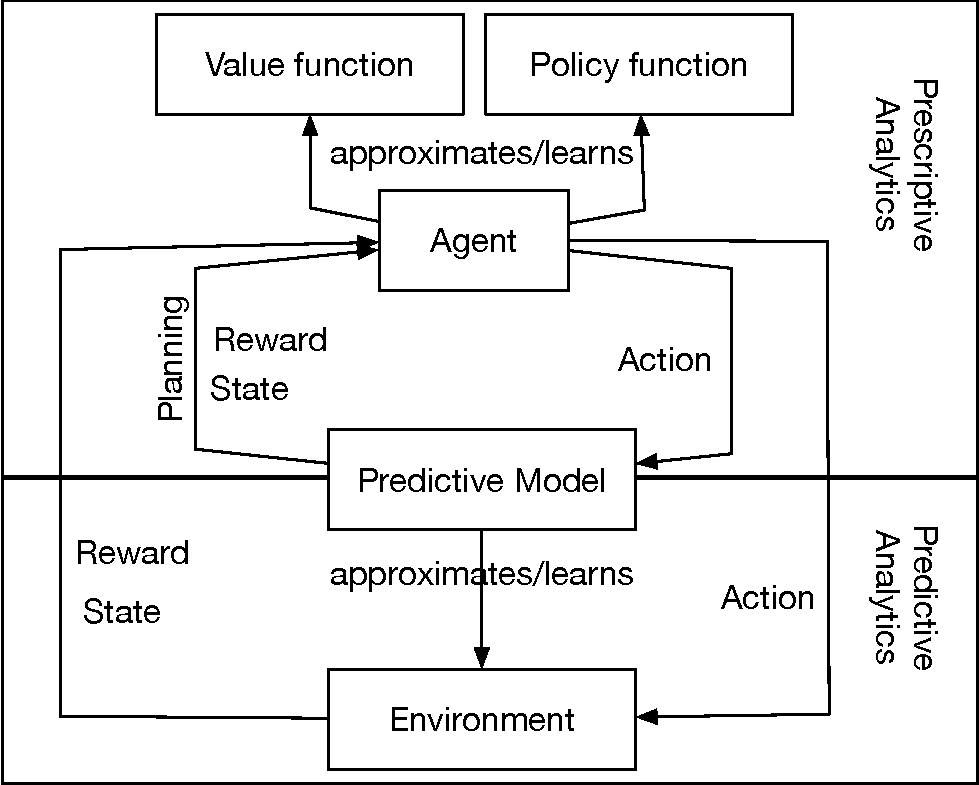
\includegraphics[width=0.4\textwidth]{figs/RLpolicy.pdf}
    \caption{The interplay between predictive and prescriptive analytics in policy-making.}
    \label{fig:RLpolicy}
\end{wrapfigure}

Autonomous decision-making agents tightly connect the frameworks of prescriptive and predictive analytics, leading to further research challenges. Such agents are
%An autonomous decision-making agent
often guided by a \textit{policy}: a function that examines the current state of its environment to select an action that leads to the highest possible future rewards. Figure \ref{fig:RLpolicy} illustrates how reinforcement learning agents can operate in real-world scenarios. Consider an auto-trader, which utilizes a stock time-series predictive model to simulate the effects (rewards) of different purchase decisions. This allows for a \textit{planning} phase where the agent can experiment with different decisions to approximate the \textit{value} of being in different possible states and to learn a policy that allows the agent to take an \textit{action} that leads to high-valued states. In this setup the predictive model is constantly updated from observations of the real world and the agent constantly updates its internal value and policy models to better determine which stocks to buy or sell on a daily basis.
%In this tightly connected analytical framework of prescriptive and predictive analytics,
% There are at least two key issues to address.

\subsection{Scaling the Planning Phase}


\setlength\intextsep{0pt}
\begin{wrapfigure}[12]{r}{0pt}
\centering
{\small
\begin{tabular}{clcccccc}
\attr{ID} $(i)$ & \attr{stock} & \attr{day} $(d)$ & \attr{E[price]} & \attr{price dist.} & \attr{E[gain]} $(g)$ & \attr{gain dist.}\\
\hline
1  & AAPL  & 1 & 150 & $f_1(1, ...)$ & 8 & $g_1(1, ...)$\\
1  & AAPL  & 2 & 158 & $f_1(2, ...)$ & 12 & $g_1(2, ...)$\\
%& ... & & && \\
1  & AAPL  & 3 & 170 & $f_1(3, ...)$ & 10 & $g_1(3, ...)$\\
2  & TSLA  & 1 & 758 & $f_2(1, ...)$ & -4 & $g_2(1, ...)$\\
2  & TSLA  & 2 & 754 & $f_2(2, ...)$ & -10 & $g_2(2, ...)$\\
%& $\cdots$ & & && \\
2  & TSLA  & 3 & 744 & $f_2(3, ...)$ & -20 & $g_2(3, ...)$\\
& && $\cdots$  &&\\
% 2  & TSLA  &Tech & 758 & $\cdots$ & ? \\
% 2  & TSLA  &Tech & 2400 & $\cdots$ & ? \\
% 2 &  TSLA  &Tech & 42 & $\cdots$ & ? \\
% 6  & GOOG  &Tech & 2280 & $\cdots$ & ? \\
% 7  & ADBE  &Tech & 415 & $\cdots$ & ? \\
% 8  & FB    &Tech & 194 & $\cdots$ & ? \\
\hline
\end{tabular}}
%\vspace{-4mm}
\caption{Predicted stock prices over a three-day horizon. VG functions $f_{i}(d, ...)$, and $g_{i}(d, ...)$ describe the uncertainty of the price and of the gain of a stock $i$ on day $d$.}
\label{tab:30daystock}
\end{wrapfigure}

An auto-trader (the agent) has an astronomical combination of decisions to consider over the planning time horizon. If the auto-trader hopes to maximize profits over a three day time horizon, it explores for each day in that period the predicted price and gain of a certain stock and how many units it should buy or sell. This exploration allows the auto-trader to construct a policy that maximizes expected profit given the current state of stock prices today and expected daily gains. If the stock prediction model updates on a daily basis, planning may need to occur in a relatively short time frame before the stock exchanges open for trading. For even more aggressive hourly traders, planning may need to occur within minutes. State-of-the-art reinforcement learning (RL) techniques such as Soft-Actor Critic (SAC) or Proximal Policy Optimization (PPO) and their variants are computationally intensive involving many simulations to construct policies. This planning phase is a bottleneck to enabling interactive policy making. 


\smallskip\textit{Reformulating Planning as a Stochastic Package Query:} One approach is to replace RL methods, such as SAC or PPO, with stochastic package query formulations. In the case of the auto-trader, the predictive model is used to build a relation similar to the one in Figure~\ref{tab:30daystock}.

The agent can construct a stochastic package query that decides how many stocks to buy or sell (short) given constraints on the principal budget and subsequent estimated daily profits. The \spaql query is similar to the one introduced in Section \ref{sec:spaql} with a buy/sell decision variable associated with each stock for each day in the planning time horizon and with the following additional constraints: 
\begin{sqlquery}
\>\>$\SUM{\attr{price \times (day=2)}} \le 50{,}000 - \SUM{\attr{price \times (day\leq1)}} + \SUM{\attr{gain \times (day\leq1)}} $ \AND\\
\>\>$\SUM{\attr{price \times (day=3)}} \le 50{,}000 - \SUM{\attr{price \times (day\leq2)}} + \SUM{\attr{gain \times (day\leq2)}} $
\end{sqlquery}
This reformulation allows us to reuse many of the discussed techniques for scaling stochastic packages directly. 

\subsection{Tracking and Explaining Policy Changes}

As the predictive model updates, so does the agent's value and policy models and subsequently the actions taken by the agent. In many situations, a human may wish to interrogate the autonomous agent to understand its reasons for choosing a certain action, especially if the action differs from past actions taken in similar states. To enable this form of \textit{why-so} questioning, we need to build a provenance system that tracks and connects changes across the predictive model and the agent's value and policy models. The ability to answer simple why questions through provenance will form the basic building blocks of interpretability and explainability in prescriptive analytical frameworks.

%%%%%%%%%%%%%%%%%%%%%%%%%%%%%%%%%%%%%%%%%%%%%%%%%%%%%%%%%%%%%%%%%%%%%%%%%%%%
%%%%%%%%%%%%%%%%%%%%%%%%%%%%%%%%%%%%%%%%%%%%%%%%%%%%%%%%%%%%%%%%%%%%%%%%%%%%

\section{Conclusions}
\label{sec:concl}

Prescriptive analytics plays a key role in a broad variety of domains, but has received relatively little attention from the database community. As optimization problems become increasingly data-intensive, database researchers are poised to make key contributions to the creation of scalable, seamless, data-centric tools for supporting decision making in complex, uncertain, dynamic environments. Our work on one useful class of optimization problems, package queries, has demonstrated the challenges and opportunities arising from the deep integration of data management, predictive analytics, and optimization software and algorithms. Many challenges remain, both in exploring a broad class of optimization problems arising in applications, and in building systems that enable improved, data-driven decision making.

%%%%%%%%%%%%%%%%%%%%%%%%%%%%%%%%%%%%%%%%%%%%%%%%%%%%%%%%%%%%%%%%%%%%%%%%%%%%
%%%%%%%%%%%%%%%%%%%%%%%%%%%%%%%%%%%%%%%%%%%%%%%%%%%%%%%%%%%%%%%%%%%%%%%%%%%%
   
    \smallskip
\noindent
   \textbf{Acknowledgments.}
  This material is based upon work supported by the ASPIRE Award for Research Excellence (AARE-2020) grant AARE20-307, the NYUAD Center for Interacting Urban Networks (CITIES), and funded by: Tamkeen under the NYUAD Research Institute Award CG001, and the National Science Foundation under grants IIS-1453543 and IIS-1943971. We thank Matteo Brucato, Riddho Haque, Anh Mai, and Nishant Yadav for their many contributions to this work.
  
%%%%%%%%%%%%%%%%%%%%%%%%%%%%%%%%%%%%%%%%%%%%%%%%%%%%%%%%%%%%%%%%%%%%%%%%%%%%
%%%%%%%%%%%%%%%%%%%%%%%%%%%%%%%%%%%%%%%%%%%%%%%%%%%%%%%%%%%%%%%%%%%%%%%%%%%%
{\small   
\begin{thebibliography}{10}

\bibitem{alkhamis2004simulation}
T.~M. Alkhamis and M.~A. Ahmed.
\newblock Simulation-based optimization using simulated annealing with
  confidence interval.
\newblock In {\em Proc. Winter Simulation Conference}, 2004.

\bibitem{alrefaei1999simulated}
M.~H. Alrefaei and S.~Andrad{\'o}ttir.
\newblock A simulated annealing algorithm with constant temperature for
  discrete stochastic optimization.
\newblock {\em Management science}, 45(5):748--764, 1999.

\bibitem{alrefaei2005discrete}
M.~H. Alrefaei and S.~Andrad{\'o}ttir.
\newblock Discrete stochastic optimization using variants of the stochastic
  ruler method.
\newblock {\em Naval Research Logistics (NRL)}, 52(4):344--360, 2005.

\bibitem{AJP+10}
S.~Arumugam, R.~Jampani, L.~Perez, F.~Xu, C.~Jermaine, and P.~J. Haas.
\newblock {MCDB-R}: Risk analysis in the database.
\newblock In {\em VLDB}, pages 782--793, 2010.

\bibitem{barton2020tutorial}
R.~R. Barton.
\newblock Tutorial: {M}etamodeling for simulation.
\newblock In {\em Proc. Winter Simulation Conference (WSC)}, pages 1102--1116,
  2020.

\bibitem{BrucatoAM18}
M.~Brucato, A.~Abouzied, and A.~Meliou.
\newblock Package queries: efficient and scalable computation of high-order
  constraints.
\newblock {\em {VLDB} J.}, 27(5):693--718, 2018.

\bibitem{BrucatoBAM16}
M.~Brucato, J.~F. Beltran, A.~Abouzied, and A.~Meliou.
\newblock Scalable package queries in relational database systems.
\newblock {\em {PVLDB}}, 9(7):576--587, 2016.

\bibitem{BrucatoMAHM20}
M.~Brucato, M.~Mannino, A.~Abouzied, P.~J. Haas, and A.~Meliou.
\newblock {sPaQLTooLs}: {A} stochastic package query interface for scalable
  constrained optimization.
\newblock {\em Proc. {VLDB} Endow.}, 13(12):2881--2884, 2020.

\bibitem{BrucatoAHM2020}
M.~Brucato, N.~Yadav, A.~Abouzied, P.~J. Haas, and A.~Meliou.
\newblock Stochastic package queries in probabilistic databases.
\newblock In {\em Proceedings of the ACM SIGMOD International Conference on
  Management of Data (SIGMOD)}, pages 269--283, 2020.

\bibitem{Cai+13}
Z.~Cai, Z.~Vagena, L.~L. Perez, S.~Arumugam, P.~J. Haas, and C.~M. Jermaine.
\newblock Simulation of database-valued {M}arkov chains using {SimSQL}.
\newblock In {\em SIGMOD}, pages 637--648, 2013.

\bibitem{CenH22}
W.~Cen and P.~J. Haas.
\newblock Enhanced simulation metamodeling via graph and generative neural networks.
\newblock In {\em 2022 Winter Simulation Conference}, to appear.

\bibitem{onion}
Y.-C. Chang, L.~Bergman, V.~Castelli, C.-S. Li, M.-L. Lo, and J.~R. Smith.
\newblock The onion technique: Indexing for linear optimization queries.
\newblock {\em SIGMOD Rec.}, 29(2):391–402, May 2000.

\bibitem{FrazzettoDPS19}
D.~Frazzetto, T.~Dyhre~Nielsen, T.~Pedersen, and L.~Siksnys.
\newblock Prescriptive analytics: a survey of emerging trends and technologies.
\newblock {\em The VLDB Journal}, May 2019.
\newblock DOI: 10.1007/s00778-019-00539-y.

\bibitem{glynn1990likelihood}
P.~W. Glynn.
\newblock Likelihood ratio gradient estimation for stochastic systems.
\newblock {\em CACM}, 33(10):75--84, 1990.

\bibitem{HaasMST11}
P.~J. Haas, P.~P. Maglio, P.~G. Selinger, and W.~C. Tan.
\newblock Data is dead... without what-if models.
\newblock {\em {PVLDB}}, 4(12):1486--1489, 2011.

\bibitem{JampaniXWPJH11}
R.~Jampani, F.~Xu, M.~Wu, L.~L. Perez, C.~Jermaine, and P.~J. Haas.
\newblock {The Monte Carlo Database System: Stochastic analysis close to the
  data}.
\newblock {\em {ACM} Trans. Database Syst.}, 36(3):18:1--18:41, 2011.

\bibitem{JampaniXWPJH08}
R.~Jampani, F.~Xu, M.~Wu, L.~L. Perez, C.~M. Jermaine, and P.~J. Haas.
\newblock {MCDB}: a {M}onte {C}arlo approach to managing uncertain data.
\newblock In {\em SIGMOD}, pages 687--700, 2008.

\bibitem{Lam2021neural}
H.~Lam and H.~Zhang.
\newblock Neural predictive intervals for simulation metamodeling.
\newblock In {\em Proc. Winter Simulation Conference (WSC)}, 2021.

\bibitem{LustigDJD10}
I.~Lustig, B.~Dietrich, C.~Johnson, and C.~Dziekan.
\newblock The analytics journey.
\newblock {\em Analytics Magazine}, November/December 2010.

\bibitem{McNeilFE15}
A.~J. McNeil, R.~Frey, and P.~Embrechts.
\newblock {\em Quantitative Risk Management: Concepts, Techniques and Tools}.
\newblock Princeton University Press, second edition, 2015.

\bibitem{norkin1998branch}
V.~I. Norkin, G.~C. Pflug, and A.~Ruszczy{\'n}ski.
\newblock A branch and bound method for stochastic global optimization.
\newblock {\em Mathematical programming}, 83(1):425--450, 1998.

\bibitem{peng2018new}
Y.~Peng, M.~C. Fu, J.-Q. Hu, and B.~Heidergott.
\newblock A new unbiased stochastic derivative estimator for discontinuous
  sample performances with structural parameters.
\newblock {\em Operations Research}, 66(2):487--499, 2018.

\bibitem{PerezAJ10}
L.~L. Perez, S.~Arumugam, and C.~M. Jermaine.
\newblock Evaluation of probabilistic threshold queries in {MCDB}.
\newblock In {\em SIGMOD}, pages 687--698, 2010.

\bibitem{SiksnysP16}
L.~Siksnys and T.~B. Pedersen.
\newblock {SolveDB}: Integrating optimization problem solvers into {SQL}
  databases.
\newblock In {\em SSDBM}, pages 14:1--14:12, 2016.

\bibitem{SiksnysPNF21}
L.~Siksnys, T.~B. Pedersen, T.~D. Nielsen, and D.~Frazzetto.
\newblock {SolveDB+}: Sql-based prescriptive analytics.
\newblock In {\em Proc. EDBT}, pages 133--144, 2021.

\bibitem{silverman2018density}
B.~W. Silverman.
\newblock {\em Density estimation for statistics and data analysis}.
\newblock Routledge, 2018.

\bibitem{smith2006optimizer}
J.~E. Smith and R.~L. Winkler.
\newblock The optimizer's curse: Skepticism and post-decision surprise in
  decision analysis.
\newblock {\em Management Science}, 52(3):311--322, 2006.

\bibitem{suciu2011probabilistic}
D.~Suciu, D.~Olteanu, C.~R{\'e}, and C.~Koch.
\newblock {\em Probabilistic Databases}.
\newblock Synthesis Lectures on Data Management. Morgan \& Claypool, 2011.

\bibitem{vanderbei2020linear}
R.~J. Vanderbei.
\newblock {\em Linear Programming: Foundations and Extensions}.
\newblock Springer Nature, 2020.

\bibitem{xiao2014simulation}
H.~Xiao and L.~H. Lee.
\newblock Simulation optimization using genetic algorithms with optimal
  computing budget allocation.
\newblock {\em Simulation}, 90(10):1146--1157, 2014.

\end{thebibliography}
}

\end{document}